\newpage
\chapter{SYSTEM DESIGN}

%------------------------------------------------
\section{PROPOSED SYSTEM}

\hspace{1cm}\textbf{Hybrid Phishing Defense} is an intelligent AI-powered cybersecurity assistant designed to monitor, analyze, and detect malicious web URLs in real time. It leverages feature extraction and deep learning techniques to identify and block zero-day phishing attempts, helping individuals browse safely and effectively without the constant reliance on centralized security vendors.

The system uses advanced deep learning architectures such as \textit{CNN} and \textit{LSTM} to identify key lexical anomalies, track structural URL patterns, and analyze host-based metadata across web sessions. Through these insights, \textbf{Hybrid Phishing Defense} provides users with immediate feedback on domain safety, ensuring that every web request aligns with legitimate structural patterns.

The platform integrates a \textbf{Decentralized Threat Registry} that learns from global performance data and dynamically logs confirmed threats to an immutable ledger. By combining real-time visual feedback, AI-based threat prediction, and blockchain analytics, \textbf{Hybrid Phishing Defense} creates a personalized, secure, and interactive browsing environment.

Additionally, the system provides real-time risk dashboards, threat intelligence sharing, and wallet integrations to help users secure their digital assets efficiently. The system supports multi-platform accessibility across Chromium-based browsers while ensuring that user browsing data is processed securely and privately.

%------------------------------------------------
\section{ARCHITECTURE}

\hspace{1cm}The architecture of \textbf{Hybrid Phishing Defense} is designed around modular integration of natural language processing, artificial intelligence, and blockchain components. The system begins with browser input that captures the user's navigated URLs in real time.

The captured URL strings are processed by the feature extraction module, which detects 89 distinct lexical and statistical data points. These results are forwarded to the CNN-LSTM inference module, which evaluates structural accuracy and determines whether a phishing alert is required.

The Decentralized Threat Registry processes positive threat data and generates smart contract transactions to record the URL. All threat records and performance metrics are stored in the Ethereum Sepolia blockchain for future analysis and global reporting.

\begin{figure}[htbp]
\centering
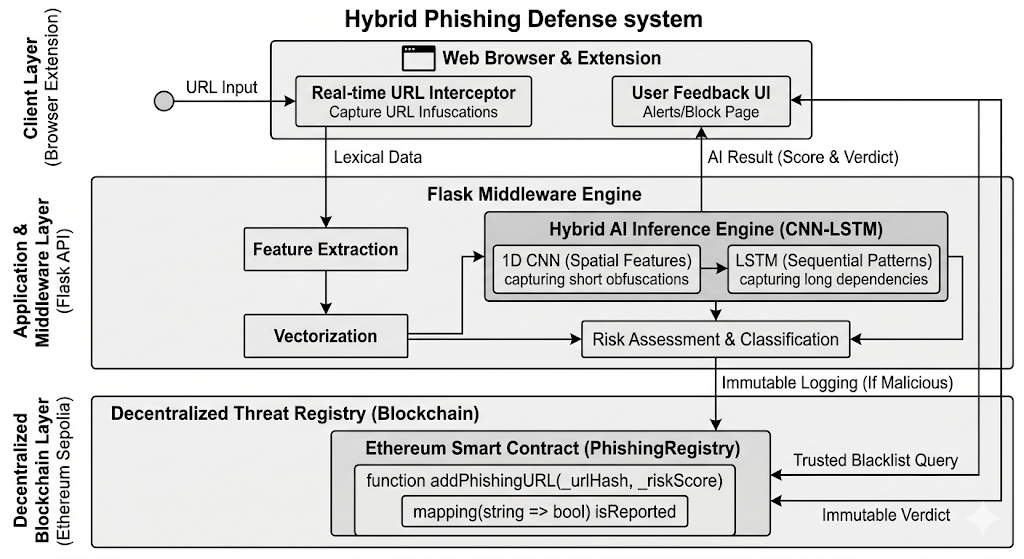
\includegraphics[width=0.9\textwidth]{assets/Architecture.png}
\caption{\centering Architecture of the proposed Hybrid Phishing Defense system}
\end{figure}

\subsection{MIDDLEWARE \& BLOCKCHAIN MODULE}

The Middleware \& Blockchain Module provides centralized processing and decentralized storage for the \textbf{Hybrid Phishing Defense} platform. The Flask backend and Smart Contracts manage threat intelligence, process URL datasets, and evaluate system analytics.

The middleware configures AI feedback parameters, updates feature extraction datasets, and monitors prediction accuracy reports. The module interacts with the CNN-LSTM engine and the Ethereum blockchain to maintain system integrity and decentralized consensus.

\subsection{CLIENT EXTENSION MODULE}

The Client Extension Module provides the main interaction interface for individuals using the \textbf{Hybrid Phishing Defense} system. Users can install the extension, navigate the web, and receive real-time feedback about their browsing security.

The system captures URL navigation through background scripts and analyzes them using the connected AI APIs. If phishing deviations are detected, the system provides visual overlays and transaction signing prompts.

Users can also view global threat reports, scan history, and risk score recommendations through the interactive dashboard.

\newpage
%------------------------------------------------
\section{MODULE DESCRIPTION}

\subsection{MIDDLEWARE \& BLOCKCHAIN MODULE}

\begin{itemize}

\item \textbf{Description}

The Middleware \& Blockchain Module acts as the core processing interface for the AI model and the distributed ledger. It allows the system to manage incoming scan requests, assign risk thresholds, and monitor global threat performance.

The backend infrastructure configures AI inference parameters, handles Web3 RPC connections, and maintains the smart contract logic used by the threat registry. This module also provides analytical data related to zero-day discoveries and network performance.

\item \textbf{Purpose}

The purpose of this module is to enable the AI engine to process data efficiently, maintain an immutable threat dataset, and ensure that the blockchain-based security platform operates smoothly.

Furthermore, the Middleware \& Blockchain Module supports system monitoring and threat evaluation by providing detailed analytical endpoints. These endpoints allow the system to observe global phishing trends, transaction completion statistics, and prediction accuracy across the network. By analyzing these metrics, the system can identify potential zero-day patterns, refine CNN-LSTM feedback models, and ensure that the platform continuously delivers accurate and effective protection to users. It also enables the network to quickly detect adversarial evasion attempts and optimize classification performance through data-driven adjustments.

\end{itemize}

\begin{figure}[htbp]
\centering
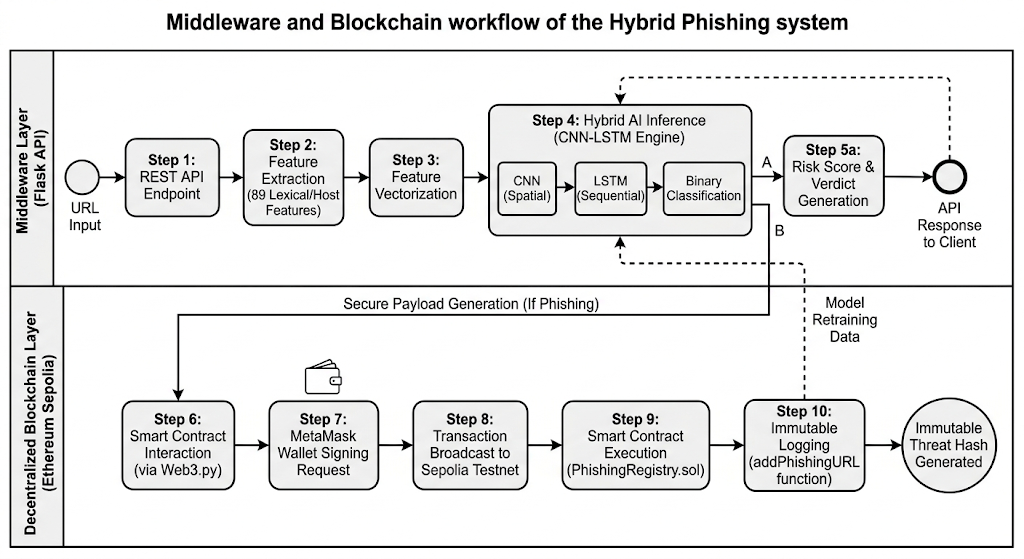
\includegraphics[width=0.9\textwidth]{assets/Backend.png}
\caption{\centering Middleware and Blockchain workflow of the Hybrid Phishing system}
\end{figure}

\textbf{Key Features}

\begin{itemize}
\item Secure API routing and Web3 integration
\item Threat logging and smart contract management
\item Inference analytics and reporting
\item Configuration of CNN-LSTM feedback mechanisms
\item Integration with the Decentralized Threat Registry
\end{itemize}
\newpage

\subsection{CLIENT EXTENSION MODULE}

\begin{itemize}

\item \textbf{Description}

The Client Extension Module provides an intuitive and user-friendly interface that enables individuals to interact effectively with the \textbf{Hybrid Phishing Defense} system. Through this module, users can install the browser extension, connect their MetaMask wallets, and configure their personal security profiles. Users can view security metrics such as sites scanned, threats blocked, and wallet connection status. The system also allows users to view specific threat parameters tailored to their browsing habits, ensuring that the security experience remains transparent and engaging.

During web browsing sessions, the system continuously monitors the user’s navigated URLs using real-time background scripts and API requests. The captured URL structures are analyzed to evaluate safety and legitimacy. If an obfuscated domain or zero-day phishing attempt is detected, the system immediately generates corrective feedback through visual overlays, popup alerts, or immediate page blocks. This real-time assistance helps users adjust their browsing instantly, reducing the risk of credential theft and improving security effectiveness.

The Client Extension Module also integrates a comprehensive security dashboard that displays detailed scan history, risk score accuracy, and threat trends over time. Users can track their protection metrics across multiple sessions through graphs, statistics, and global summaries. Additionally, the system provides MetaMask signing prompts, safe browsing recommendations, and ledger feedback to encourage consistent security habits and long-term asset protection.

The module also supports interactive functionality by adapting visual alerts based on the severity of the AI risk score. This adaptive behavior ensures that interventions remain suitable for the threat level while gradually improving user awareness, operational security, and overall browsing safety.

\end{itemize}

\begin{figure}[htbp]
\centering
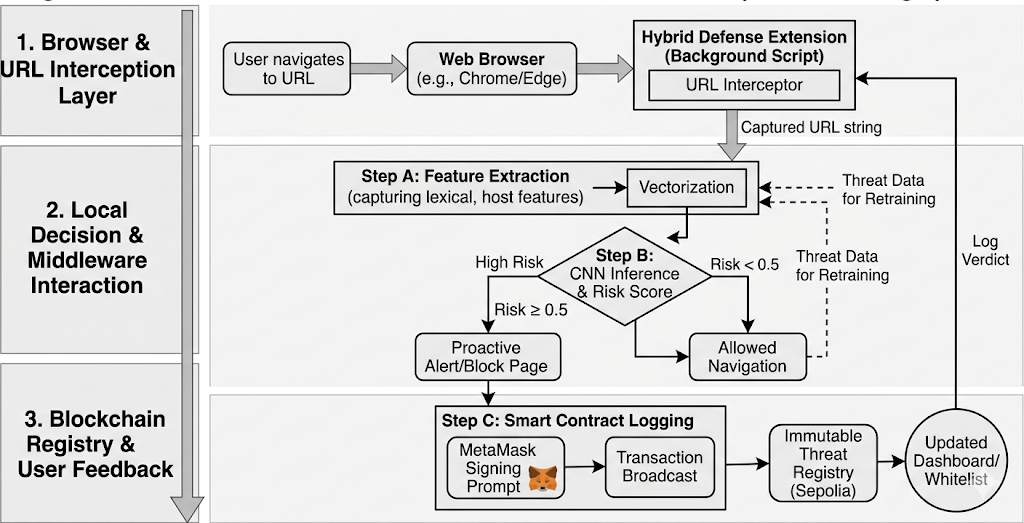
\includegraphics[width=0.85\textwidth]{assets/Client.png}
\caption{\centering Client Extension interface and workflow of the Hybrid Phishing system}
\end{figure}

\newpage
\textbf{Key Features}

\begin{itemize}
\item Real-time URL interception and scanning
\item AI-driven visual alerts and page blocking
\item MetaMask wallet signing integration
\item Threat tracking and decentralized analytics
\item Secure local storage and connection management
\end{itemize}
 \newpage
%------------------------------------------------
\section{DATA FLOW DIAGRAM}

Data Flow Diagrams illustrate how information moves through the Hybrid Phishing Defense system.

\subsection{MIDDLEWARE \& BLOCKCHAIN MODULE}

\textbf{Level 0}

\begin{figure}[htbp]
\centering
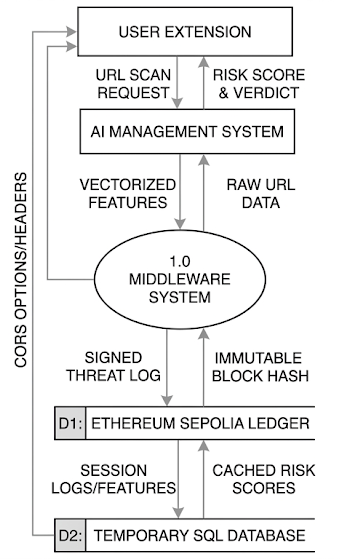
\includegraphics[width=0.7\textwidth]{assets/DFD_Backend_L0.png}
\caption{\centering Level 0 Data Flow Diagram of Middleware Module}
\end{figure}
\newpage
\textbf{Level 1}

\begin{figure}[htbp] 
    \centering
    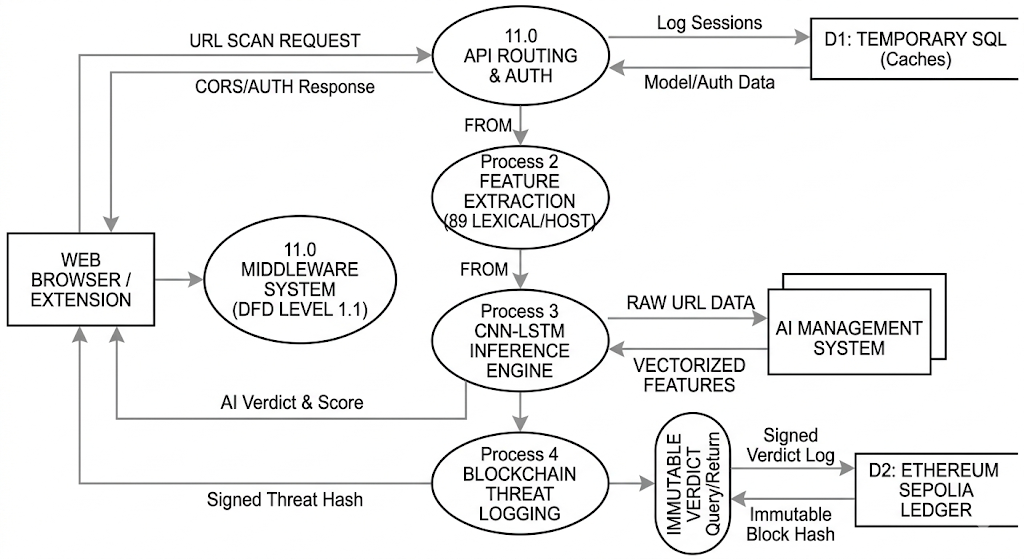
\includegraphics[width=0.9\textwidth]{assets/DFD_Backend_L1.png}
    \caption{\centering Level 1 Data Flow Diagram of Middleware Module}
    \label{fig:dfd_backend}
\end{figure}

\noindent The Level 0 and Level 1 Data Flow Diagrams collectively describe how security data is processed within the \textbf{Hybrid Phishing Defense} system. The Level 0 diagram provides a simplified overview where the Middleware interacts with the AI Management System to perform tasks such as feature extraction, prediction, and Web3 routing while data is stored in the blockchain ledger. The Level 1 diagram expands this view by illustrating internal system components such as data parsing, AI inference routing, smart contract execution, and transaction verification modules. These modules interact with the Decentralized Threat Registry and the Ethereum network to process security operations efficiently and maintain immutable records of identified threats and system performance.

\newpage
\subsection{CLIENT EXTENSION MODULE}
\textbf{Level 0}

The Level 0 Data Flow Diagram (DFD) of the Client Module illustrates the main interaction between the user and the \textbf{Hybrid Phishing Defense} system. In this diagram, the user provides inputs such as URL navigation, wallet connection, and signing approvals to the Browser Interaction System. The system processes this information and communicates with the Middleware \& Blockchain component to evaluate and log data. Based on the processed information, the system provides outputs such as block pages, risk scores, and dashboard insights to the user.

\begin{figure}[htbp]
\centering
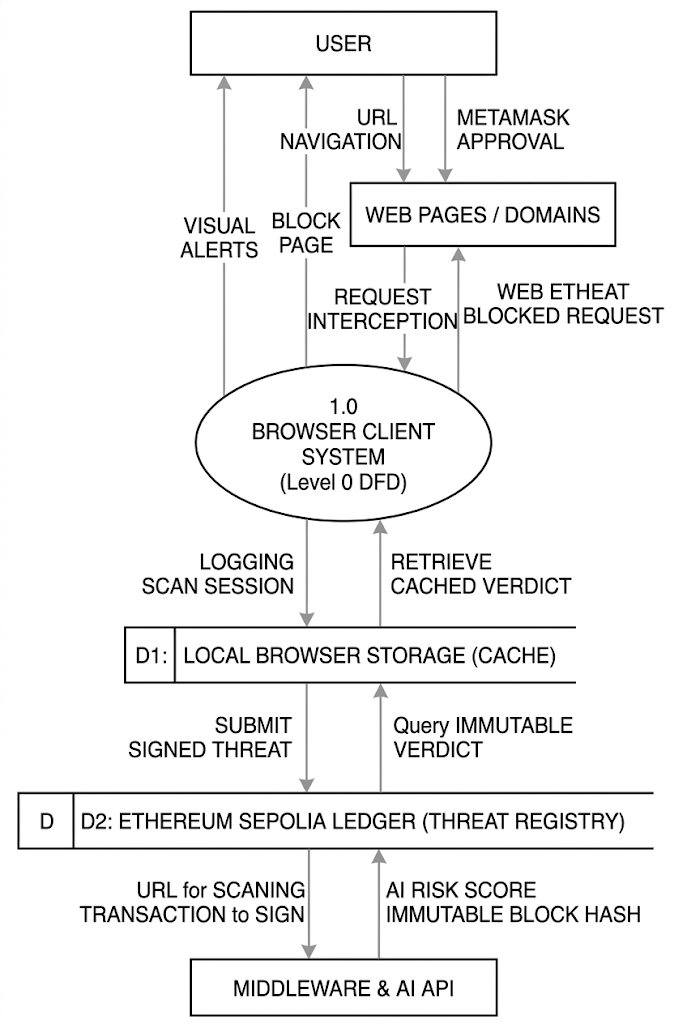
\includegraphics[width=0.75\textwidth]{assets/DFD_Client_L0.png}
\caption{\centering Level 0 Data Flow Diagram of Client Module}
\end{figure}

\noindent\textbf{Level 1}

\noindent The Level 1 Data Flow Diagram of the Client Module illustrates the internal workflow of the \textbf{Hybrid Phishing Defense} system, starting from URL interception and MetaMask setup to real-time risk evaluation and alert generation. The process includes background script capture, API communication, AI risk assessment, smart contract interaction, and transaction storage in the decentralized ledger.  

It also demonstrates how URL metrics are analyzed to generate visual overlays and wallet prompts. The processed security data is finally stored in the global blockchain system for tracking community threat intelligence and future analysis.

\begin{figure}[htbp]
\centering
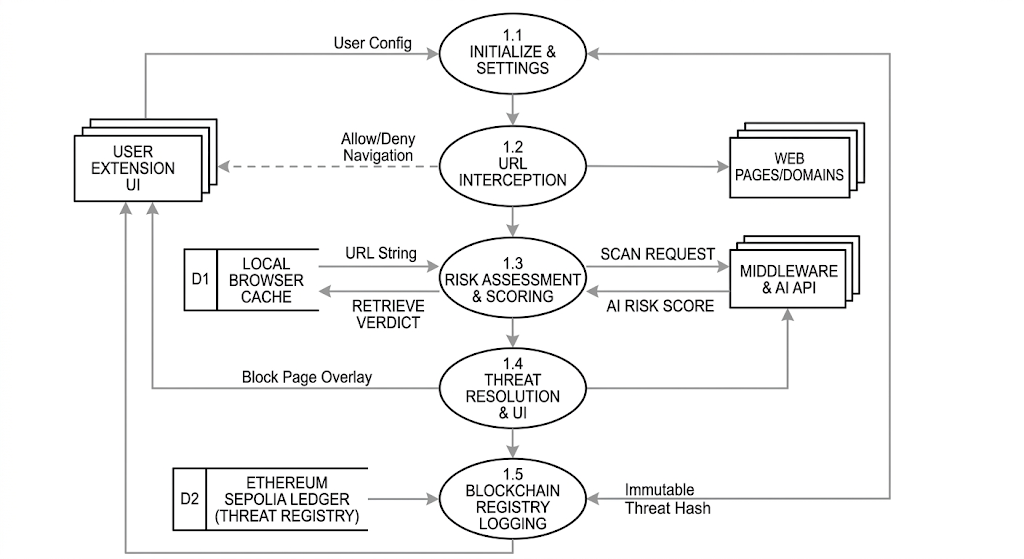
\includegraphics[width=0.9\textwidth]{assets/DFD_Client_L1.png}
\caption{\centering Level 1 Data Flow Diagram of Client Module}
\end{figure}

\newpage

%------------------------------------------------
\section{ER DIAGRAM}

The Entity Relationship (ER) diagram illustrates the data structure of the \textbf{Hybrid Phishing Defense} system. It defines the relationship between users, URL scans, and the decentralized threat registry.

The \textbf{Users} entity stores the wallet address and connection details of interacting users.

The \textbf{Scans} entity stores URL session records including the raw URL, extracted features, AI risk score, and timestamps.

The \textbf{Registry} entity manages the smart contract logging, transaction hashes, and global threat records.

\begin{figure}[htbp]
\centering
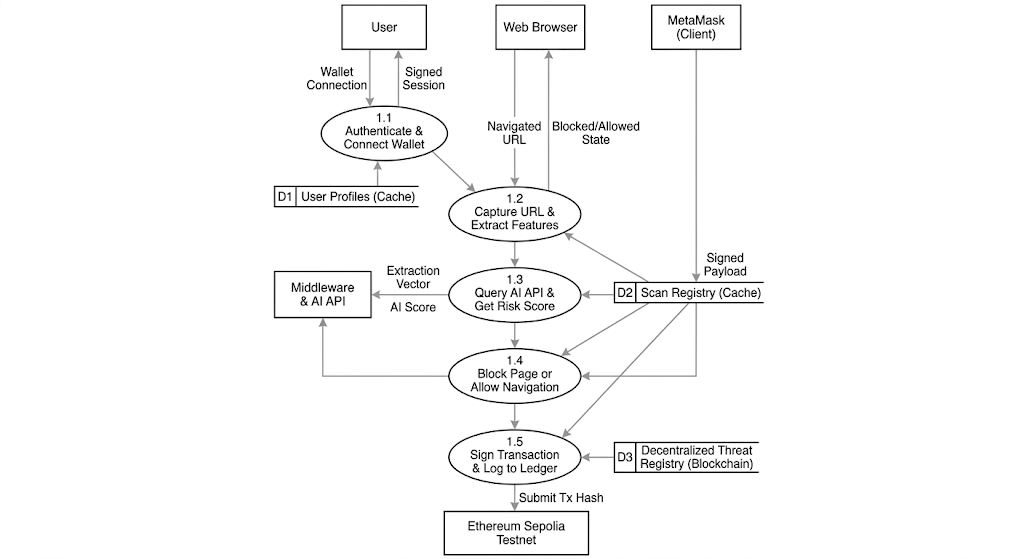
\includegraphics[width=0.95\textwidth]{assets/ER.png}
\caption{\centering Entity Relationship Diagram of Hybrid Phishing System}
\end{figure}

%------------------------------------------------
\section{LANGUAGES \& TOOLS}

The \textbf{Hybrid Phishing Defense} system is implemented using modern programming languages, frameworks, and tools suitable for AI-based lexical monitoring, real-time threat analysis, and decentralized data interaction. These technologies enable the system to process real-time web data, perform feature extraction, and generate intelligent smart-contract transactions during browsing sessions. The combination of deep learning frameworks and modern Web3 technologies ensures that the platform remains scalable, tamper-proof, and capable of supporting future enhancements. This technological combination allows the platform to deliver accurate, real-time security monitoring and decentralized threat assistance.

\begin{itemize}

\item \textbf{Programming Languages}
\begin{itemize}[label=*]
\item Python 3.9+
\item Solidity
\item JavaScript / TypeScript
\end{itemize}

\item \textbf{Technology Stack}
\begin{itemize}[label=*]
\item React (Frontend Dashboard)
\item Flask (Python Middleware)
\item Ethereum Sepolia Testnet
\end{itemize}

\item \textbf{Frameworks and Libraries}
\begin{itemize}[label=*]
\item TensorFlow / Keras
\item Web3.py / Ethers.js
\item NumPy / Pandas
\item Flask-CORS
\end{itemize}

\item \textbf{APIs and Intelligent Services}
\begin{itemize}[label=*]
\item Infura / Alchemy (Ethereum RPC endpoints)
\end{itemize}

\item \textbf{Development Tools}
\begin{itemize}[label=*]
\item Visual Studio Code
\item Hardhat / Remix IDE
\item MetaMask
\end{itemize}

\item \textbf{Database}
\begin{itemize}[label=*]
\item Decentralized Smart Contract Storage (Ethereum)
\item LocalStorage (Browser Extension State)
\end{itemize}

\end{itemize}